
The Complex number equivalent to the matrix is: 

\begin{align}
\myvec{a & -b\\ b & a } \implies \myvec{a \\ b }
\end{align}
 
\begin{align}
 \vec{A}  = \myvec{ a \\ b }\implies \vec{A}^\top = \myvec{a \\ -b}  
\end{align}



And addition of $\vec{A}$ with $\vec{A}^\top$ results in  :
  
\begin{align}
    \myvec{  a \\ b } + \myvec{ a \\ -b } = \myvec{ 2a \\ 0}
\end{align}
So, According to the given question $\vec{A}$ + $\vec{A}^\top$ is : 
\begin{align}
   \myvec{\cos{\alpha} \\ \sin{\alpha}} + \myvec{\cos{\alpha} \\ -\sin{\alpha}} = \myvec{ 2\cos{\alpha} \\ 0} 
\end{align}

Given that  $\vec{A}$ + $\vec{A}^\top$ = $\vec{I}$ :
\begin{align}
  \myvec{2\cos{\alpha} \\ 0} = \myvec{ 1 \\ 0} 
\end{align}

That Implies, 
\begin{align}
 2\cos{\alpha} = 1 \implies \cos{\alpha} = \frac{1}{2}   
\end{align}

As per the cosine values, the angle $\alpha$ is :
\begin{align}
 \alpha =  \frac{\pi}{3} = 1.047
\end{align}
  
%The cosine function is plotted along with the point (x, cos(x)) = (1.047, 0.5) as shown in Fig. 0:  
%\begin{figure}[h]
%    \centering
%    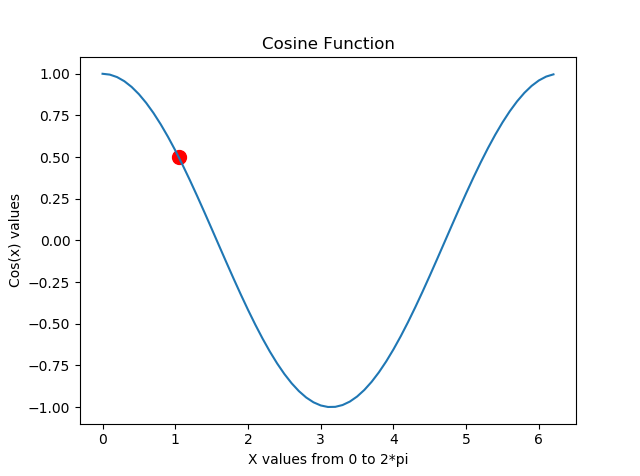
\includegraphics[width=\columnwidth]{assignment_2.png}
%    \caption{Cosine Function}
%    \label{fig:cosine}
%\end{figure}
